\documentclass[a4paper]{article}

\addtolength{\hoffset}{-2.25cm}
\addtolength{\textwidth}{4.5cm}
\addtolength{\voffset}{-3.25cm}
\addtolength{\textheight}{5cm}
\setlength{\parskip}{0pt}
\setlength{\parindent}{0in}

%----------------------------------------------------------------------------------------
%	PACKAGES AND OTHER DOCUMENT CONFIGURATIONS
%----------------------------------------------------------------------------------------

\usepackage{blindtext} % Package to generate dummy text
\usepackage{charter} % Use the Charter font
\usepackage[utf8]{inputenc} % Use UTF-8 encoding
\usepackage{microtype} % Slightly tweak font spacing for aesthetics
\usepackage[english]{babel} % Language hyphenation and typographical rules
\usepackage{amsthm, amsmath, amssymb} % Mathematical typesetting
\usepackage{float} % Improved interface for floating objects
\usepackage[final, colorlinks = true,
            linkcolor = black,
            citecolor = black]{hyperref} % For hyperlinks in the PDF
\usepackage{graphicx, multicol} % Enhanced support for graphics
\usepackage{xcolor} % Driver-independent color extensions
\usepackage{marvosym, wasysym} % More symbols
\usepackage{rotating} % Rotation tools
\usepackage{censor} % Facilities for controlling restricted text
\usepackage{listings} % Environment for non-formatted code, !uses style file!
\usepackage{pseudocode} % Environment for specifying algorithms in a natural way
 % Environment for f-structures, !uses style file!
\usepackage{booktabs} % Enhances quality of tables
\usepackage{tikz-qtree} % Easy tree drawing tool
 % Configuration for b-trees and b+-trees, !uses style file!
\usepackage[backend=biber,style=numeric,
            sorting=nyt]{biblatex} % Complete reimplementation of bibliographic facilities
\addbibresource{ecl.bib}
\usepackage{csquotes} % Context sensitive quotation facilities
\usepackage[yyyymmdd]{datetime} % Uses YEAR-MONTH-DAY format for dates
\renewcommand{\dateseparator}{-} % Sets dateseparator to '-'
\usepackage{fancyhdr} % Headers and footers
\pagestyle{fancy} % All pages have headers and footers
\fancyhead{}\renewcommand{\headrulewidth}{0pt} % Blank out the default header
\fancyfoot[L]{} % Custom footer text
\fancyfoot[C]{} % Custom footer text
\fancyfoot[R]{\thepage} % Custom footer text
\newcommand{\note}[1]{\marginpar{\scriptsize \textcolor{red}{#1}}} % Enables comments in red on margin
\usepackage{mathtools}
\usepackage{amsmath}
\DeclarePairedDelimiter\abs{\lvert}{\rvert}%
\usepackage{cancel}
\usepackage{minted}
\usepackage{float}
%-------------------------------

%----------------------------------------------------------------------------------------

%-------------------------------
%	ENVIRONMENT SECTION
%-------------------------------
\pagestyle{fancy}
\usepackage{mdframed}


\newenvironment{problem}[2][Problema]
    { \begin{mdframed}[backgroundcolor=gray!20] \textbf{#1 #2} \\}
    {  \end{mdframed}}

% Define solution environment
\newenvironment{solution}
    {\textit{Solución}}
    {}


%-------------------------------------------------------------------------------------------
%	CUSTOM COMMANDS
%-------------------------------
\newcommand{\gaussian}{\frac{1}{\sigma\sqrt{2\pi}}\exp\left(- \frac{(x-\mu)^2}{2\sigma^2}\right)}
\newcommand{\R}{\mathbb R}

\def\inline{\lstinline[basicstyle=\ttfamily,keywordstyle={}]}


\begin{document}


%-------------------------------
%	TITLE SECTION
%-------------------------------

\fancyhead[C]{}
\hrule \medskip % Upper rule
\begin{minipage}{0.295\textwidth}
\raggedright
\footnotesize
Francisco Javier Sáez Maldonado \hfill\\
77448344F \hfill\\
franciscojavier.saez@estudiante.uam.es
\end{minipage}
\begin{minipage}{0.4\textwidth}
\centering
\large
Ejercicios Bootstrap\\
\normalsize
Métodos Avanzados en Estadística\\
\end{minipage}
\begin{minipage}{0.295\textwidth}
\raggedleft
\today\hfill\\
\end{minipage}
\medskip\hrule
\bigskip

%-------------------------------
%	CONTENTS
%-------------------------------





\begin{problem}{2}
  Sea \( X_1,\dots,X_n\) una muestra de \(n\) observaciones iid de una distribución \(F\) con \(\mu\) y varianza \(\sigma^2\), y sea \(X_1^*,\dots,X_n^*\) una muestra de \(n\) observaciones iid de la distribución empírica de la muestra irignial \(F_n\). Calcula las siguientes cantidades:

  \begin{enumerate}
  \item \(E_{F_n}( \bar X_n^* ):= E(\bar X_n^* \ | X_1,\dots,X_n)\)
  \item \(E_F(\bar{X_n^*})\)
  \item \(Var_{F_n}\left(\bar X_n^*\right) := Var(\bar X_n^* \ | X_1,\dots, X_n)\)
  \item \(Var_F(\bar X_n^*)\)


    \end{enumerate}
  \end{problem}

   \begin{enumerate}

     \item \(E_{F_n}( \bar X_n^* ):= E(\bar X_n^* \ | X_1,\dots,X_n)\).\\

  Basta ver que, usando la definición y la linealidad de la esperanza,
  \[
  E_{F_n}\left( \bar{X^*_n}\right) = E_{F_n}\left[\frac{1}{n} \sum_{i=1}^n X_i^* \right] = \frac{1}{n} \sum_{i=1}^n E_{F_n} \left[X_i^*\right].
  \]
  Ahora, La esperanza bajo la función de distribución empírica de los \( X_i^*\) es la misma para todos los \(i\), porlo que podemos decir que estamos decir que estamos sumando \(n\) veces la esperanza de \(X_i^*\) habiendo fijado un \(i\). Tenemos por tanto:
  \[
  \frac{1}{n} \sum_{i=1}^n E_{F_n} \left[X_i^*\right] = E_{F_n}\left[X_i^*\right] = \sum_{x \in (X_1,\dots,X_n)} P(x) x  = \sum_x \frac{1}{n} x = \bar x
  \]

\item \(E_F(\bar{X_n^*})\).\\

  Ahora no tenemos un condicionamiento como lo teníamos anteriormente, pero podemos usar la fórmula de la probabilidad total y ver que:
  \begin{align*}
    E_F(\bar{X_n^*}) & = E_f \left[ E_{F_n}(X_n^*|X_1,\dots,X_n)\right] \\
    & = E_F[\bar X] \\
    & = E_F\left[ \frac{1}{n}\sum_{i=1}^n X_i\right] \\
    & = \frac{1}{n}\sum_{i=1}^n E_F[X_i]\\
    & = \frac{n\mu}{n} \\
    & = \mu
  \end{align*}



\item \(Var_{F_n}\left(\bar X_n^*\right) := Var(\bar X_n^* \ | X_1,\dots, X_n)\).\\

  Desarrollamos primeramente igual que en el primer caso:
  \begin{align*}
  Var_{F_n}\left(\bar X_n^*\right) &:= Var_{F_n}(\bar X_n^* \ | X_1,\dots, X_n)\\
    & = Var_{F_n}\left(\frac{1}{n} \sum_{i=1}^n X_i^* \ | X_1,\dots,X_n\right)\\
    & =  \frac{1}{n^2} \sum_{i=1}^n Var_{F_n}(X_i^* | X_1,\dots, X_n ) \\
    & =  \frac{n}{n^2} Var_{F_n}(X_i^* | X_1,\dots,X_n),
  \end{align*}
  donde, en la última igualdad usamos que para cada una de las \(X_i^*\) la varianza bajo \(F_n\) es la misma, así que la estamos sumando \(n\) varianzas iguales. Calculamos ahora la varianza que nos ha quedado para terminar así el ejercicio:
  \begin{align*}
    \frac{1}{n}  Var(X_i^* |X_1,\dots,X_n) &  = \frac{1}{n}\left(E_{F_n}\left[\left( (X_1^*)^2 | X_1,\dots,X_n \right)\right] - E_{F_n}\left[(X_i^*|X_1,\dots,X_n)\right]^2\right) \\
    & = \frac{1}{n} \left( \left( \frac{1}{n} \sum_{i=1}^n  X_i^2\right) - \bar X^2 \right) \\
    & = \frac{1}{n^2} \left(\sum_{i=1}^n X_i^2 - \sum_{i=1}^n \bar X^2 \right)\\
    & = \frac{n-1}{n^2} \underbrace{\frac{1}{n-1} \left(\sum_{i=1}^n (X_i^2 - \bar X^2) \right)}_{s^2}
  \end{align*}
  Por lo que, obtenemos finalmente que
  \[
  Var_{F_n}(\bar X_{n}^*) = \frac{n-1}{n^2}s^2
  \]


\item  \(Var_F(\bar X_n^*)\).\\
  Para este último apartado, utilizamos la fórmula de la varianza iterada del siguiente modo:
  \begin{align*}
    Var_F(\bar X_n^*) &= E_F\left[ Var_{F_n}(\bar X_n^*|X_1,\dots,X_n)\right] + Var_F\left(E_{F_n}(\bar X_n^*|X_1,\dots,X_n)\right) \\
    & = E_F\left[\frac{n-1}{n^2}s^2\right] + Var_F(\bar X) \\
    & = \frac{n-1}{n^2} E_F[s^2] + Var_F\left( \frac{1}{n} \sum_{i=1}^n  X_i\right) \\
  \end{align*}
  Ahora, sabemos que \(E_F[s^2] = \sigma^2\) por lo que
  \begin{align*}
    \frac{n-1}{n^2} E_F[s^2] + Var_F\left( \frac{1}{n} \sum_{i=1}^n  X_i\right) & =  \frac{n-1}{n^2}\sigma^2 + \frac{1}{n^2} n Var_F{X_i}\\
    & = \frac{n-1}{n^2}\sigma^2 + \frac{1}{n}\sigma^2 \\
    & = \frac{2n-1}{n^2}\sigma^2
  \end{align*}

   \end{enumerate}




   \begin{problem}{7}
     Sea \(F\) una distribución con media \(\mu\), varianza \(\sigma^2\) y coeficiente de asimetría
     \[
     \gamma = E_F[(X-\mu)^3]/\sigma^3.
     \]
     Genera \(R=1000\) muestras de observaciones iid \(X_1,\dots,X_n\) con \(X_i \equiv N(0,1)\) para \(n=100\). Para cada una de ellas, calcula tres intervalos de confianza bootstrap de nivel \(95\%\) para \(\gamma\) usando el método híbrido, el método normal y el método percentil. Determina el porcentaje de intervalos que contienen al parámetro en cada caso. Repite el ejercicio con muestras procedentes de una distribución exponencial de parámetro \(\lambda=1\).
   \end{problem}

   Vamos a proceder a resolver el ejercicio de la forma más general posible. Adjuntaremos todo el código para dar comodidad al lector por si quiere ahorrarse ejecutarlo.\\

   Lo primero que hacemos, aunque no sea muy importante, es crear una función que, pasándole como parámetro una función, nos devuelva una muestra de tamaño \(n\) de la distribución que representa la función que le hemos dado como parámetro. Está programada para la distribución normal y la distribución exponencial, que son las que usaremos en este ejercicio, pero podrían añadirse más distribuciones. Además, inicializamos los parámetros iniciales para el experimento:
   \begin{minted}{R}
     set.seed(234)
R <- 1000     # número de remuestras
mu <- 0
sigma <- 1
n <- 100
alpha <- 0.05
m <- 100
theta <- 0
generate_sample <- function(distr){
  if(identical(distr,rnorm)){
    return (rnorm(n,mu,sigma))
  }
  else{
    return (rexp(n,rate=1))
  }
}
   \end{minted}

   Ahora, para reducir el tamaño del bucle principal y poder reutilizar el código, escribimos funciones que nos calculen el intervalo de confianza y si el parámetro queda dentro del intervalo de confianza. Realizamos una para cada método:
   \begin{minted}{R}
hybrid_ci_gen <- function(bootstrap_samples, original_estimator,bootstrap_estimator){
  # Obtain final T
  T_bootstrap <- sqrt(n) * (bootstrap_estimator - original_estimator)

  # Compute confidence interval
  ci_min <- original_estimator -  quantile(T_bootstrap, 1-alpha/2)/sqrt(n)
  ci_max  <- original_estimator -  quantile(T_bootstrap, alpha/2)/sqrt(n)
  interval <-  c(ci_min, ci_max)
  # Obtain accuracy
  accuracy <-  ci_min < theta & ci_max > theta

  return(list(interval,accuracy))
}

# Function that computes the confidence interval
# using the percentile method. Same parameters.
percentile_ci_gen <- function(bootstrap_samples, original_estimator,bootstrap_estimator){

  #Obtain confidence interval
  ci_min <- quantile(bootstrap_estimator, alpha/2)
  ci_max <- quantile(bootstrap_estimator,1-alpha/2)
  interval <-  c(ci_min, ci_max)
  # Obtain accuracy
  accuracy <-  ci_min < theta & ci_max > theta

  return(list(interval,accuracy))
}

# Function that computes the confidence interval
# using the normal method. Same parameters.
normal_ci_gen <- function(bootstrap_samples, original_estimator,bootstrap_estimator){
  #Obtain confidence interval
  ci_1 <- original_estimator - qnorm(alpha/2,0,1)*sd(bootstrap_estimator)
  ci_2 <- original_estimator + qnorm(alpha/2,0,1)*sd(bootstrap_estimator)
  ci_min <- min(ci_1,ci_2)
  ci_max <- max(ci_1,ci_2)
  interval <-  c(ci_min, ci_max)
  # Obtain accuracy
  accuracy <-  ci_min < theta & ci_max > theta

  return(list(interval,accuracy))
}
     \end{minted}


   Una vez tenemos estas funciones, solo tenemos que en cada una de las \(m\) repeticiones, generar \(R\) muestras bootstrap y calcular los intervalos de confianza para cada una de ellas, usando las funciones en cuestión. Creamos una función que, pasándole como parámetro una función que sea la que queremos usar para generar la muestra inicial, nos haga este proceso.

   \begin{minted}{R}
compute_ci <- function(distr){
  hybrid_intervals <- NULL
  hybrid_acc <- NULL
  normal_intervals <- NULL
  normal_acc <- NULL
  percentile_intervals <- NULL
  percentile_acc <- NULL

  for (i in 1:m){
    # Obtain original data and original T
    original_data <- generate_sample(distr)
    original_skew <- skewness(original_data)

    # Obtain bootstrap sample and bootstrap estimator
    bootstrap_data <- sample(original_data,n*R,rep = TRUE)
    bootstrap_data <- matrix(bootstrap_data, nrow = n)
    bootstrap_skew <- apply(bootstrap_data, 2, skewness)

    # Obtain ci and accuracy value for this iteration
    res_hybrid <- hybrid_ci_gen(bootstrap_data, original_skew, bootstrap_skew)
    res_normal <- normal_ci_gen(bootstrap_data, original_skew, bootstrap_skew)
    res_percentile <- percentile_ci_gen(bootstrap_data, original_skew, bootstrap_skew)

    hybrid_intervals <- rbind(hybrid_intervals,res_hybrid[[1]])
    hybrid_acc <- rbind(hybrid_acc,res_hybrid[[2]])

    normal_intervals <- rbind(normal_intervals, res_normal[[1]])
    normal_acc <- c(normal_acc,res_normal[[2]])

    percentile_intervals <- rbind(percentile_intervals, res_percentile[[1]])
    percentile_acc <- c(percentile_acc, res_percentile[[2]])

  }


  hybrid_total_acc <- sum(hybrid_acc == TRUE) / length(hybrid_acc)
  normal_total_acc <- sum(normal_acc == TRUE) / length(normal_acc)
  percentile_total_acc <- sum(percentile_acc == TRUE) / length(percentile_acc)

  print(sprintf("Acc for hybrid: %f", hybrid_total_acc))
  print(sprintf("Acc for normal: %f", normal_total_acc))
  print(sprintf("Acc for percentile: %f", percentile_total_acc))


  plot_interval(hybrid_intervals,hybrid_acc,"híbrido")
  plot_interval(normal_intervals,normal_acc,"suposicion normal")
  plot_interval(percentile_intervals,percentile_acc,"percentil")

}
   \end{minted}

   Tras esto, tenemos nuestros resultados listos para poder obtener el porcentaje de acierto y dibujar los gráficos correspondientes. Además, hemos creado una función que encapsula el dibujado de los gráficos de los intervalos de confianza. El código es sencillo.

   \begin{minted}{R}
plot_interval <- function(intervals,acc,name){
  df <- data.frame(ic_min <- intervals[,1],
                   ic_max <- intervals[, 2],
                   ind = 1:m,
                   acierto = acc)
  p <- ggplot(df) +
    geom_linerange(aes(xmin = ic_min, xmax = ic_max, y = ind, col = acc)) +
    scale_color_hue(labels = c("NO", "SÍ")) +
    geom_vline(aes(xintercept = theta), linetype = 2) +
    theme_bw() +
    labs(y = 'Muestras', x = 'Intervalos (nivel 0.95)',
         title = sprintf('IC (método bootstrap %s)',name))

  print(p)
}
   \end{minted}

   Hemos modularizado bastante, de modo que todo sea más cómodo de realizar y podamos incluso reutilizar código en futuras ocasiones. Para ejecutarlo, lo hacemos cómodamente del siguiente modo:
   \begin{minted}{R}
theta <- 0
print("Accuracies for the gaussian distribution")
solutions <- compute_ci(rnorm)

theta <-2
print("Accuracies for the exponential distribution")
solutions <- compute_ci(rexp)
   \end{minted}

   Y queda así ejecutado para las dos distribuciones que queríamos probar. Vemos que tenemos que cambiar el parámetro \(\theta\) pues en la distribución exponencial es \(2\). Sabemos además que este coeficiente de simetría es siempre \(2\) para la distribución exponencial de cualquier parámetro \(\lambda\). Si lo ejecutamos, obtenemos:
   \begin{minted}{bash}
[1] "Accuracies for the gaussian distribution"
[1] "Acc for hybrid: 0.910000"
[1] "Acc for normal: 0.940000"
[1] "Acc for percentile: 0.950000"


[1] "Accuracies for the exponential distribution"
[1] "Acc for hybrid: 0.580000"
[1] "Acc for normal: 0.680000"
[1] "Acc for percentile: 0.630000"
   \end{minted}

   A priori, los resultados obtenidos en la distribución gaussiana parecen buenos, mientras que los de la función exponencial quedan bastante lejos de aproximar bien al parámetro. Además, los gráficos obtenidos son los siguientes:

   \begin{figure}[!htb]
\minipage{0.32\textwidth}
  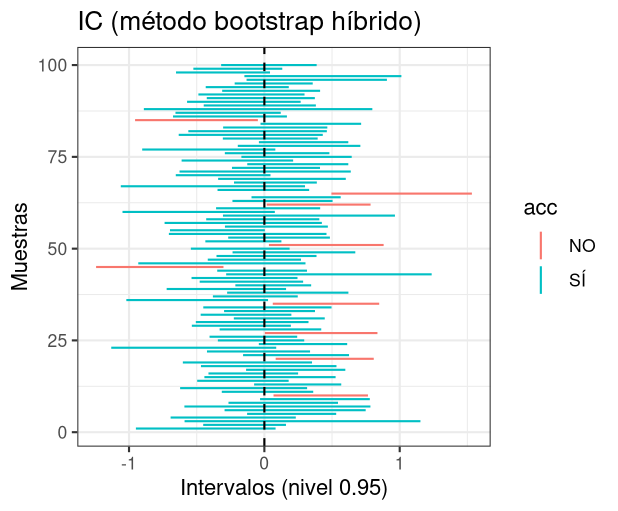
\includegraphics[width=\linewidth]{media/norm-hybrid.png}
\endminipage\hfill
\minipage{0.32\textwidth}
  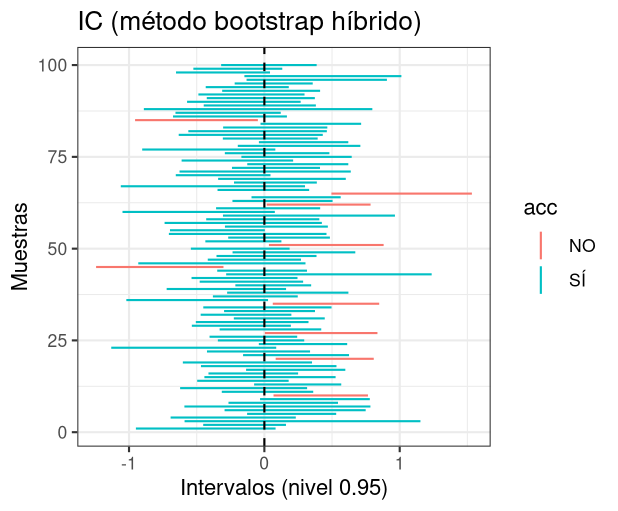
\includegraphics[width=\linewidth]{media/norm-hybrid.png}
\endminipage\hfill
\minipage{0.32\textwidth}%
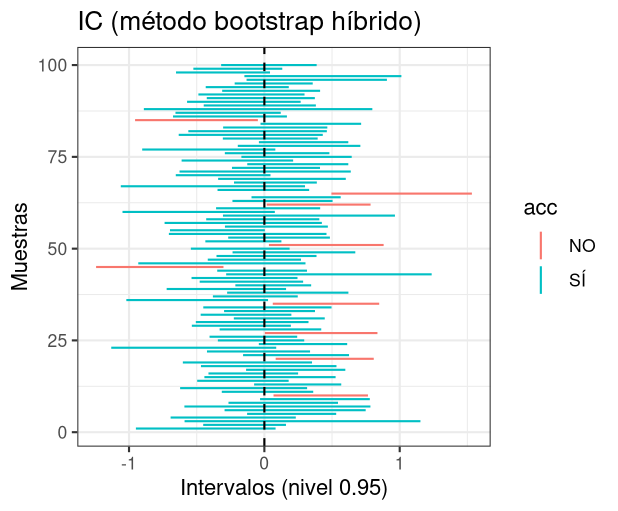
\includegraphics[width=\linewidth]{media/norm-hybrid.png}
\endminipage
\caption{Resultados usando la distribución normal}
   \end{figure}

    \begin{figure}[H]
\minipage{0.32\textwidth}
  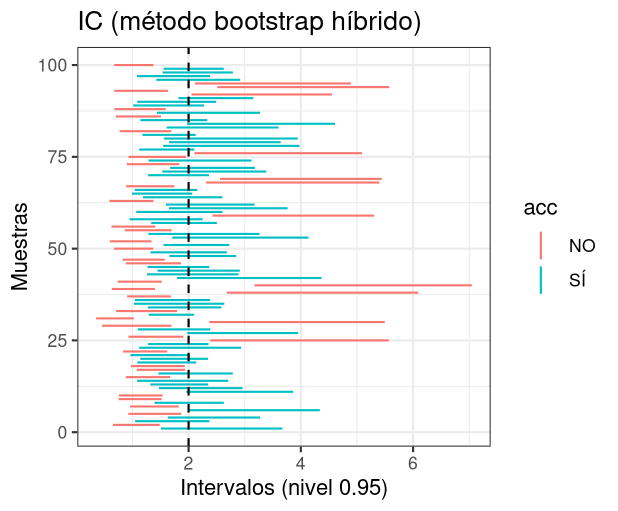
\includegraphics[width=\linewidth]{media/rexp-hybrid.png}

\endminipage\hfill
\minipage{0.32\textwidth}
  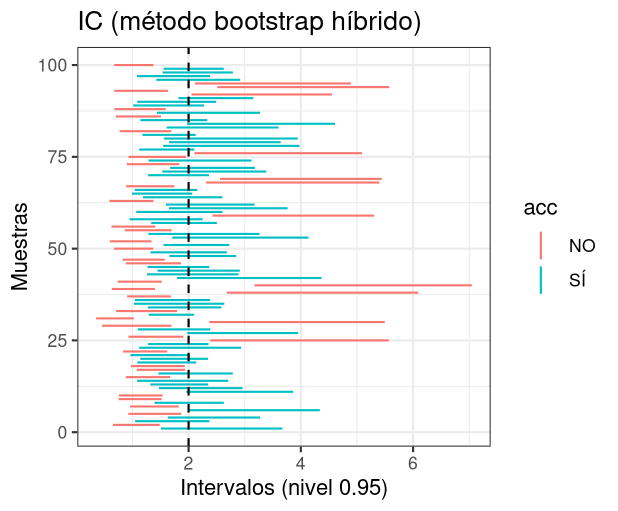
\includegraphics[width=\linewidth]{media/rexp-hybrid.png}

\endminipage\hfill
\minipage{0.32\textwidth}%
  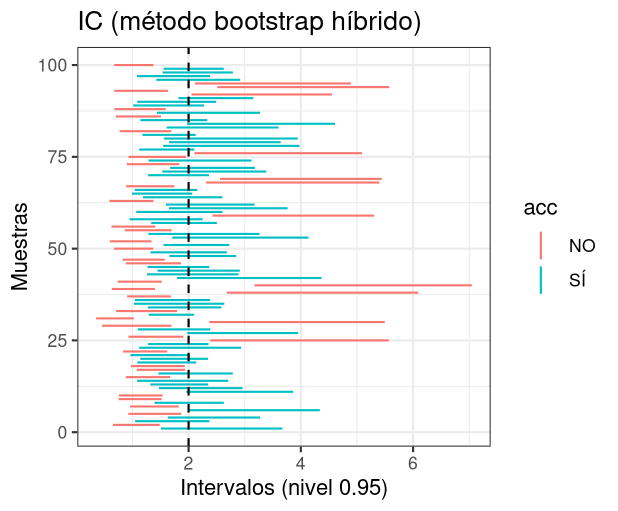
\includegraphics[width=\linewidth]{media/rexp-hybrid.png}
  \endminipage
  \caption{Resultados usando la distribución exponencial}
  \end{figure}

Estos gráficos representan lo que ya nos indicaba el porcentaje de acierto incial. Vemos que hemos conseguido estimar mediante bootstrap de forma razonablemente buena el coeficiente de asimetría de la normal, mientras que nos hemos quedado lejos de conseguir lo mismo en la función exponencial. Podría estar ocurriendo que el bootstrap no sea el mejor método para estimar la distribución de este estadístico.

\end{document}
